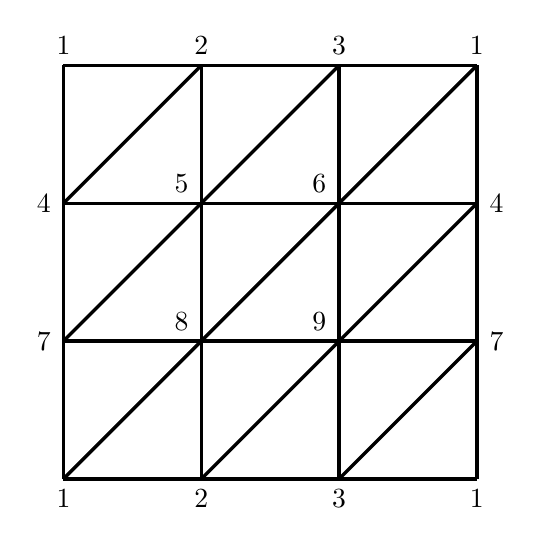
\begin{tikzpicture}
	\def \unit{1.75}
	\def \sep{0.25}
	\foreach \x in {0,1,...,3}{\draw[very thick] (\unit*\x, 0) -- (\unit*\x, 3*\unit);\draw[very thick] (0, \unit*\x) -- (3*\unit, \unit*\x);};
	\foreach \x in {0,1,...,2}{\draw[very thick] (0, \unit*\x) -- ({(3-\x)*\unit}, {3*\unit}); \draw[very thick] (\x*\unit, 0) -- ({3*\unit}, {(3-\x)*\unit});};
	% row 1
	\foreach \x in {1,2,...,3}{\node[] at ({(\x-1)*\unit}, 3*\unit+\sep) {$\x$};}; % top 1 2 3
	\node[] at (3*\unit, 3*\unit+\sep) {$1$};
	% row 2
	\node[] at (-\sep, 2*\unit) {$4$};
	\node[] at (\unit-\sep, 2*\unit+\sep) {$5$};
	\node[] at (2*\unit-\sep, 2*\unit+\sep) {$6$};
	\node[] at (3*\unit+\sep, 2*\unit) {$4$};
	% row 3
	\node[] at (-\sep, \unit) {$7$};
	\node[] at (\unit-\sep, \unit+\sep) {$8$};
	\node[] at (2*\unit-\sep, \unit+\sep) {$9$};
	\node[] at (3*\unit+\sep, \unit) {$7$};
	% row 4
	\foreach \x in {1,2,...,3}{\node[] at ({(\x-1)*\unit}, -\sep) {$\x$};}; % bottom 1 2 3
	\node[] at (3*\unit, -\sep) {$1$};
\end{tikzpicture}